\documentclass[dvipdfmx,tikz]{standalone}
\usepackage{tikz,bm}
\begin{document}
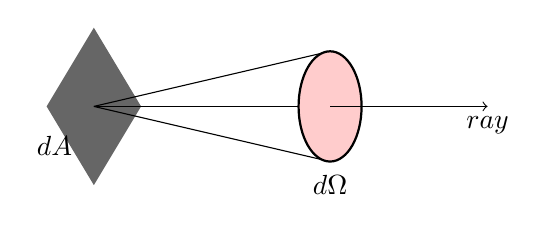
\begin{tikzpicture}
    %\draw[help lines] (-2,-1) grid (4,2);
    \node[] at(-0.5,.5) {$dA$};
    \node[] at(3,0) {$d\Omega$};
    \fill[black,opacity=.6] (0,0) -- (0.6,1) -- (0,2) -- (-0.6,1);
    \draw[](0,1) -- (2.6,1);
    \draw[](0,1) -- (3,1.7);
    \draw[](0,1) -- (3,0.3);
    \draw[thick,fill=red!20] (3,1) circle[x radius = 0.4, y radius = 0.7];
    \draw[->](3,1) -- (5,1) node[anchor=north]{$ray$};
\end{tikzpicture}
\end{document}